\chapter{高中笔记8}
\section{读书笔记}
康托尔: 德, 数学家, 集合论的创造人, 他证明了一条直线上的点和一个平面上的点一一对应, 也能和空间中的点一一对应.
因此1cm长的线段内的点与太平洋面上的点以及整个地球内部的点都``一样多". 他对这类``无穷集合"问题发表了一系列文章,
通过严格证明得出了许多惊人的结论.

罗素悖论: 又称理发师悖论: 某村只有一人会理发, 且该村的人都需要理发, 理发师约定, 给且只给村中自己不给自己理发的人理发, 
试问: 理发师给不给自己理发.

阿贝尔: 椭圆函数论的创始人之一, 发现了椭圆函数的加法定理, 双周期性. 在交换群, 二项级数的严格理论, 级数求和等有巨大贡献,
还有阿贝尔积分, 阿贝尔积分方程, 阿贝尔函数, 阿贝尔级数, 阿贝尔部分和公式, 阿贝尔收敛判别法, 阿贝尔可和性.

分形: 龙的曲线是由一个等腰直角三角形开始的, 以该等腰直角三角形的直角边为斜边作另外的等腰直角三角形, 如此往后, 
并将其斜边删除掉即可.

群论: 伽罗瓦是第一个使用群并系统地研究群的数学家. 他19岁时, 用群的思想解决了五次方程的问题. 逐渐开创了一个新的数学分支--抽象代数学.
它包括群论, 环论, 域论, 布尔代数等.

说谎者悖论: 公元前4世纪, 希腊哲学家也提出:``我现在正在说的这句话是谎话". 另外公元前6世纪,
古希腊克里特鸟的哲学家伊壁门尼德斯断言:``所有克里特人所说的每一句话都是谎话."

干下去还有50\%成功的希望, 不干便是100\%的失败.

$A=x+y+z$($A$:成功, $x$: 艰苦的劳动, $y$: 正确的方法, $z$: 少说空话)--爱因斯坦的公式.

埃托色尼的筛法提的求小于给定数$N$的所有素数的方法: 先从3写出所有小于$N$的奇数, 
再从中划去$3, 5, 7, 11\cdots$的倍数.

球体填充问题: 把一大堆乒乓球倒进一个箱内, 倒至最后还剩几个, 使箱内乒乓球数目最多. 称为球体填充问题, 亦称开普勒猜想.

查: 吴文俊的``吴示性类", ``吴示嵌类".

药剂师的砝码: 将300g药粉分成100g和200g各一份, 可是天平只有30g和35g两个砝码, 只需分两次即可, 分两步:
一, 将30g砝码放一盘上, 把300g药粉倒在两个盘上, 使之平衡, 于是, 一盘药粉为165g, 另一盘135g; 第二步将35g砝码, 
从135g药粉中称出35g$\cdots$.

罗氏几何的公理系统与欧氏几何公理不同之处是: 平行公理: ``用直线外一点, 至少可做两条直线与已知直线平行"来代替,
这引出了一连串和欧氏几何内容不同的新的几何命题.

\section{球面几何}
\bd{大圆}{}
一个过球心的平面在球面上的截线叫做球面上的一个大圆.
\ed

\bd{球面二面角}{}
球面上任两个大圆都相交于对顶的两点, 一对对顶点与连接它们的两条大圆弧(半个大圆弧)围成的图形称为球面二面角(梭形).
\ed

\bd{球面角}{}
球面上一点及过该点的任意两条大圆弧所构成的图形称为球面角, 这两条大圆弧的切线间的夹角即为该球面角的大小.
\ed

\bd{球面三角形}{}
在半径为$R$的球面上相距小于$\pi R$的给定三点$A, B, C$唯一地确定了三条小于半圆的大圆圆弧$\wideparen{AB}, \wideparen{BC}, \wideparen{CA}$.
\ed

\bd{伴垂心}{}
如下左图是$\triangle ABC$的垂心的定义, 如下右图与$\triangle ABC$全等, 若$B'D'=CD$, $C'E'=AE$, $AF=B'F'$, 则$\triangle A'B'C'$中的三线共点$H'$为$\triangle A'B'C'$的伴垂心.

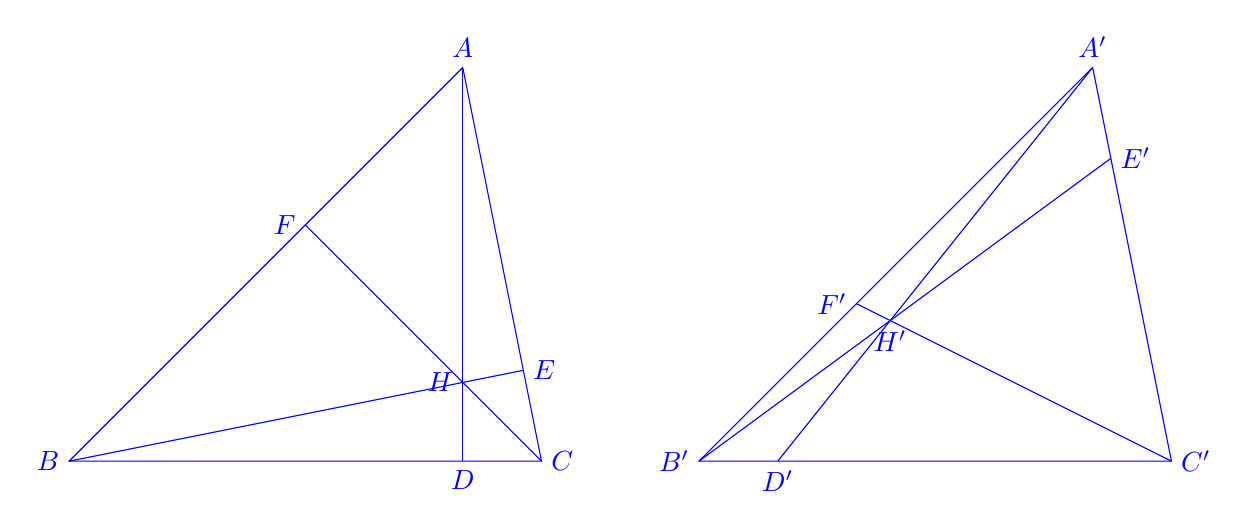
\begin{tikzpicture}
 \coordinate [label=above:\textcolor{blue}{$A$}] (A) at (5,5);
 \coordinate [label=left:\textcolor{blue}{$B$}] (B) at (0,0);
 \coordinate [label=right:\textcolor{blue}{$C$}] (C) at (6,0);
 \coordinate [label=below:\textcolor{blue}{$D$}] (D) at (5,0);
 \coordinate [label=left:\textcolor{blue}{$F$}](F) at (3,3);
 \coordinate [label=right:\textcolor{blue}{$E$}](E) at (150/26, 30/26);
 \coordinate [label=left:\textcolor{blue}{$H$}](H) at (5,1);
 
 \draw[blue] (A) -- (B) -- (C) -- (A);
 \draw[blue] (B) -- (E);
 \draw[blue] (C) -- (F);
 \draw[blue] (A) -- (D);
 
 \coordinate [label=above:\textcolor{blue}{$A'$}] (A') at (13,5);
 \coordinate [label=left:\textcolor{blue}{$B'$}] (B') at (8,0);
 \coordinate [label=right:\textcolor{blue}{$C'$}] (C') at (14,0);
 \coordinate [label=below:\textcolor{blue}{$D'$}] (D') at (9,0);
 \coordinate [label=left:\textcolor{blue}{$F'$}] (F') at (10,2);
 \coordinate [label=right:\textcolor{blue}{$E'$}] (E') at (172/13, 50/13);
 \coordinate [label=below:\textcolor{blue}{$H'$}] (H') at (73/7, 25/14);
 
  \draw[blue] (A') -- (B') -- (C') -- (A');
 \draw[blue] (B') -- (E');
 \draw[blue] (C') -- (F');
 \draw[blue] (A') -- (D');
\end{tikzpicture}
\ed

\bt{球面三角形余弦定理}{}
对于任给半径为$R$的球面三角形$\triangle ABC$, 其三边$a,b,c$和三角$\angle A, \angle B, \angle C$之间恒满足:
\begin{align*}
 \cos\frac{a}{R^2} & =\cos\frac{c}{R^2}\cos\frac{b}{R^2}+\sin\frac{b}{R^2}\sin\frac{c}{R^2}\cos\angle A,\\
 \cos\frac{b}{R^2} & =\cos\frac{a}{R^2}\cos\frac{c}{R^2}+\sin\frac{c}{R^2}\sin\frac{a}{R^2}\cos\angle B,\\
 \cos\frac{c}{R^2} & =\cos\frac{b}{R^2}\cos\frac{a}{R^2}+\sin\frac{a}{R^2}\sin\frac{b}{R^2}\cos\angle C.
\end{align*}
\et

\bt{球面三角形正弦定理}{}
条件同上, 有$\frac{\sin\angle A}{\sin\frac{a}{R^2}}=\frac{\sin\angle B}{\sin\frac{b}{R^2}}=\frac{\sin\angle C}{\sin\frac{c}{R^2}}$.
\et

\section{不等式集}
\bq{}{}
已知$0\le a_k\le 1$($k=1,2,\cdots, 2002$), 记$a_{2003}=a_1$, $a_{2004}=a_2$, 求$\sum_{k=1}^{2002}(a_k-a_{k+1}\cdot a_{k+2})$的最大值.
\eq
\ba
\bee
\sum_{k=1}^{2002}(a_k-a_{k+1}\cdot a_{k+2})=\sum_{k=1}^{2002}(a_k-a_{k}a_{k+1})=\sum_{k=1}^{2002}a_{k}(1-a_{k+1}).
\eee
Cauchy不等式, 上式右端不超过
\bee
\sqrt{\left(\sum_{k=1}^{2002}a_k^2\right)\left(\sum_{k=1}^{2002}(1-a_{k+1})^2\right)}
\le \frac{\sum a_k^2 + \sum (1-a_{k+1})^2}{2}
=\frac{\sum a_k^2+\sum(1-a_k)^2}{2}
=\frac{\sum(2a_k^2-2a_k+1)}{2}.
\eee
因为$2a_k^2-2a_k+1\le1$, 所以原式不超过$\frac12\sum1=1001$, 当$a_k=0$或$1$时取等号, 即当$a_1=a_3=a_5=\cdots=a_{2001}=1$且$a_2=a_4=\cdots=a_{2002}=0$时取等号.
\ea
\ba
由$0\le a_k\le 1$, 得$(1-a_k)(1-a_{k+1})=1-(a_{k}+a_{k+1})+a_{k}a_{k+1}\ge0$($k=1,2,\cdots, 2002$), 所以$1\ge a_{k}+a_{k+1}-a_{k}a_{k+1}\ge a_{k}+a_{k+1}-2a_{k}a_{k+1}$,
从而$2002\ge\sum_{k=1}^{2002}(a_k+a_{k+1}-2a_{k}a_{k+1})=2\sum(a_k-a_{k+1}a_{k+2})$, 即$\sum(a_k-a_{k+1}a_{k+2})\le1001$.
\ea

\bq{}{}
求函数$y=x+\sqrt{x(2-x)}$的最值及此时$x$的值.
\eq
\ba
显然$x\in[0,2]$, 所以可设$x=2\sin^2\theta$($\theta\in\mathbb{R}$), 运用$|a\sin\theta+b\cos\theta|\le\sqrt{a^2+b^2}$即可.
\ea

\bq{}{}
设$n$是给定的正整数, $n\ge13$, 对$n$个给定的实数$a_1, a_2, \cdots, a_n$, 记$|a_i-a_j|$($1\le i < j\le n$)有最小值$m$, 求在$\sum_{i=1}^{n}a_i^2=1$的条件下, 
$m$的最大值.
\eq
\ba
不妨设$a_1\le a_2\le \cdots\le a_n$, 于是$a_2-a_1\ge m, a_3-a_2\ge m, \cdots, a_n-a_{n-1}\ge m$, $a_j-a_i\ge(j-i)m$($1\le i< j \le n$).
\bee
\sum_{1\le i<j\le n}(a_i-a_j)^2\ge m^2\times\sum_{1\le i<j\le n}(j-i)^2
=m^2\sum_{k=1}^{n-1}k(2k+1)(k+1)=\frac{m^2}{12}\cdot n^2(n^2-1).
\eee
另一方面, $\sum_{i=1}^{n}a_i^2=1$可得
\bee
\sum_{1\le i<j\le n}(a_i-a_j)^2=n-\left(\sum_{i=1}^{n}a_i\right)^2\le n.
\eee
故$n\ge\frac{m^2}{12}n^2(n^2-1)$, 所以$m\le\sqrt{\frac{12}{n^2(n^2-1)}}$, 当且仅当$\sum_{i=1}^{n}a_i=0$,
且$a_1, a_2, \cdots, a_n$成等差数列时取等号.
\ea

\bq{}{}
若$x,y,z>0$且$x^2+y^2+z^2=1$, 则$S=\frac{(z+1)^2}{2xyz}$取最小值时, $x$的值是多少?
\eq
\ba
$\sqrt{\sqrt{2}-1}$.
\ea

\bl{}{}
设$T\ge0$, $x, y, z\ge0$, 则$T\ge\sum x$的充要条件为:
\begin{align}
 & (T^2-\sum x^2)^2-8\prod x\cdot T-4\sum y^2z^2\ge0\label{20170327001}\\
 & T^2\ge\sum x^2.\label{20170327002}
\end{align}
\el
\ba
若$T\ge\sum x$, 则\ref{20170327002}式明显成立, 且
\bee
(T+\sum x)(T^2-\sum x^2+2\sum yz)-8\prod x
\ge2\sum x\cdot 4\sum yz-8\prod x
\ge0.
\eee
根据
\be
(T^2-\sum x^2)^2-8\prod x\cdot T-4\sum y^2z^2
=(T-\sum x)\left[(T+\sum x)(T^2-\sum x^2+2\sum yz)-8\prod x\right]\label{20170327003}
\ee
知\ref{20170327001}式成立. 若\ref{20170327001}, \ref{20170327002}式成立, 则
\bee
(T+\sum x)(T^2-\sum x^2+2\sum yz)-8\prod x
\ge (\sqrt{\sum x^2}+\sum x)\cdot 2\sum yz-8\prod x
\ge (\sqrt{3}+3)(\prod x)^{\frac13}\cdot6(\prod x)^{\frac23}-8\prod x\ge0.
\eee
根据\ref{20170327003}式知$T\ge\sum x$.
\ea
由引理即得
\bt{}{20170328001}
设$T\ge0$, $x,y,z\ge0$, 记$f=(T^2-\sum x^2)^2-8\prod x\cdot T-4\sum y^2z^2$, 则
\begin{enumerate}[(i)]
 \item 若$f\ge0$, $\sum x^2\le T^2$, 则$\sum x\le T$;
 \item 若$f\le 0$, 则$\sum x\ge T$.
\end{enumerate}
\et

\bq{}{}
\bee
\sum\cos\frac{A}{2}\le2+\frac{s}{4R}+\frac{9\sqrt{3}-16}{4R}r.
\eee
\eq
\ba
设$m=\frac{s}{4R}$, $n=\frac{r}{2R}$. 则$\sum\cos^2\frac{A}{2}=2+n$, $\prod\cos\frac{A}{2}=\frac{m}{2}$. 进而
\bee
\sum\cos^2\frac{A}{2}\cos^2\frac{B}{2}=\frac14(4+4n+m^2+n^2).
\eee
令$T=2+\frac{m}{2}+\frac{9\sqrt{3}-16}{2}n$, $x=\cos\frac{A}{2}$, $y=\cos\frac{B}{2}$, $z=\cos\frac{C}{2}$,
用定理\ref{th:20170328001}中结论(i).
\ea

\bq{}{}
设实数$a,b,c,d$, 满足$a^2+b^2+c^2+d^2=5$, 求$(a-b)^2+(a-c)^2+(a-d)^2+(b-c)^2+(b-d)^2+(c-d)^2$的最大值.
\eq
\ba
设$f=(a-b)^2+(a-c)^2+(a-d)^2+(b-c)^2+(b-d)^2+(c-d)^2=15-2(ab+ac+ad+bc+bd+cd)+\lambda(a^2+b^2+c^2+d^2-5)$,
所以$f_a=-2(b+c+d)+2a\lambda$, $f_b=-2(a+c+d)+2b\lambda$, $f_c=-2(a+b+d)+2c\lambda$, $f_d=-2(a+c+d)+2b\lambda$,
$f_{\lambda}=a^2+b^2+c^2+d^2-5$, 令$f_a=f_b=f_c=f_d=f_{\lambda}=0$, 解得$\lambda=-1$或$a=b=c=d$.
当$\lambda=-1$时, $a+b+c+d=0$得$f=20$.
当$a=b=c=d$时, $f=0$, 所以$f_{\max}=20$.
\ea

\bq{}{}
如果$x>0$, $y>0$, $z>0$且$x^2+y^2+z^2=1$, 求$\frac{yz}{x}+\frac{xz}{y}+\frac{xy}{z}$的最小值.
\eq
\ba
设$\frac{yz}{x}=a$, $\frac{xz}{y}-b$, $\frac{xy}{z}=c$, 则
$ab+bc+ca=1$, 所以$a^2+b^2+c^2\ge ab+bc+ca=1$, 所以$(a+b+c)^2=a^2+b^2+c^2+2(ab+bc+ca)\ge3$,
另外令$f=a+b+c+\lambda(ab+bc+ca-1)$, 令
$f_a=1+(b+c)\lambda=0$, $f_b=1+(a+c)\lambda=0$, $f_c=1+(a+b)\lambda=0$, 所以
$a=b=c$时最小.
\ea

\bq{}{}
设$a_0, a_1, a_2, \cdots, a_n$满足$a_0=\frac12$, $a_{k+1}=a_k+\frac{1}{n}a_k^2$, $k=0,1,2,\cdots, n-1$,
其中$n$是一个给定的正整数, 试证: $1-\frac{1}{n}<a_n<1$.
\eq
\ba
$a_n>a_{n-1}>a_{n-2}>\cdots>a_2>a_1>a_0=\frac{1}{2}$,
\begin{align*}
 \frac{1}{a_k}-\frac{1}{a_{k+1}}=\frac{1}{n+a_k}<\frac{1}{n} \Longrightarrow\frac{1}{a_0}-\frac{1}{a_n}<1,\\
 \frac{1}{a_k}-\frac{1}{a_{k+1}}=\frac{1}{n+a_k}>\frac{1}{n+1} \Longrightarrow\frac{1}{a_0}-\frac{1}{a_n}>\frac{n}{n+1}.
\end{align*}
\ea

\bq{}{}
当$a>1$时, 若不等式$\frac{1}{n+1}+\frac{1}{n+2}+\cdots+\frac{1}{2n}>\frac{7}{12}\left[\log_{a+1}x-\log_{a}x+1\right]$对于不小于2的正整数$n$恒成立,
求$x$的取值范围.
\eq
\ba
$a_{n}=\frac{1}{n+1}+\frac{1}{n+2}+\cdots+\frac{1}{2n}$递增, $x$的取值范围为$(1, +\infty)$.
\ea

\bq{}{}
实数集$\{a_0, a_1, a_2, \cdots, a_n\}$, 满足以下条件: 
\begin{enumerate}[(1)]
 \item $a_1=a_n=0$.
 \item 对$1\le k\le n-1$, 有$a_k=c+\sum_{i=k}^{n-1}a_{i-k}(a_i+a_{i+1})$.
\end{enumerate}
证明: $c\le\frac{1}{4n}$.
\eq
\ba
定义$S_k=\sum_{i=0}^ka_i$($k=0,1,2,\cdots, n$), 则
\begin{align*}
 S_n
 & =\sum_{k=0}^{n}a_k
 =\sum_{k=0}^{n-1}a_{k-1}
 =nc+\sum_{k=0}^{n-1}\sum_{i=k}^{n-1}a_{i-k}(a_i+a_{i+1})\\
 & =nc+\sum_{i=0}^{n-1}(a_i+a_{i+1})\cdot\sum_{k=0}^{i}a_{i-k}\\
 & =nc+\sum_{i=0}^{n-1}(a_i+a_{i+1})\sum_{t=0}^{i}a_t, (t=i-k)\\
 & =nc+\sum_{i=0}^{n-1}(a_i+a_{i+1})\cdot S_i\\
 & =nc+\left[S_1S_0+(S_2-S_0)S_1+(S_3-S_1)S_2+\cdots+(S_n-S_{n-2})S_{n-1}\right]
\end{align*}
即$S_n^2-S_n+nc=0$, $\Delta\ge0\Longrightarrow c\le\frac{1}{4n}$.
\ea

\bq{}{}
若关于$x$的不等式$\log_{\frac{1}{a}}(\sqrt{x^2+ax+5}+1)\cdot\log_{5}(x^2+ax+6)+\frac{1}{\log_{3}a}\ge0$,
求$a$的取值范围.
\eq
\ba
令$u=x^2+ax+5$, $\frac{\log_3(\sqrt{u}+1)}{-\log_3a}\cdot\log_5(u+1)+\frac{1}{\log_3a}\ge0$.
因为$f(4)=1$, 所以$a=2$.
\ea

\bq{}{}
设$a_1, a_2, \cdots, a_{2002}>0$且$\sum\frac{1}{2+a_i}=\frac12$, 求$\prod a_i$的最小值.
\eq
\ba
令$x_i=\frac{2}{2+a_i}$, 则$\sum x_i=1$, 则$a_i=2\cdot\frac{1-x_i}{x_i}$, 
因为
\begin{align*}
 \prod a_i
 & =2^{2002}\prod\frac{1-x_i}{x_i}\\
 & =2^{2002}\cdot\frac{1}{x_1x_2\cdots x_{2002}}\prod(x_1+x_2+\cdots+x_{i-1}+x_{i+1}+\cdots+x_{2002})\\
 & \ge2^{2002}\cdot\frac{1}{x_ix_2\cdots x_{2002}}\cdot2001^{2002}\cdot\prod\sqrt[2001]{x_1x_2\cdots x_{i-1}x_{i+1}\cdots x_{2002}}\\
 &=4002^{2002}.
\end{align*}
\ea

\bq{}{}
求最小的正数$\lambda$, 使得对任意正整数$n$, $a_i$和$b_i$, $b_i\in[1,2]$($i=1,2,\cdots, n$), 且$\sum_{i=1}^{n}a_{i}^2=\sum b_i^2$, 
都有$\sum\frac{a_i^3}{b_i}\le\lambda\cdot\sum a_i^2$.
\eq
\ba
对任意$c_i, b_i\in[1,2]$, 有$\frac{1}{2}\le\frac{c_i}{b_i}\le 2$, 即$\frac{1}{2}b_i\le c_i\le2b_i$,
从而$\left(\frac{1}{2}b_i-c_i\right)(2b_i-c_i)\le0$, 即$c_i^2+b_i^2\le\frac{5}{2}c_ib_i$,
两边对$i$从1到$n$求和, 得$\sum c_i^2+\sum b_i^2\le\frac{5}{2}\sum c_ib_i$,
设$a_i, b_i\in\left[1, \frac{2}{3}\right]$, 因$a_i^2=\frac{a_i^{\frac{3}{2}}}{b_i^{\frac{1}{2}}}\cdot a_i^{\frac{1}{2}}\cdot b_i^{\frac{1}{2}}$.
又
\bee
\frac{1}{2}\le\frac{\frac{a_i^{\frac{3}{2}}}{b_{i}^{\frac{1}{2}}}}{a_i^{\frac{1}{2}}\cdot b_i^{\frac{1}{2}}}\le 2.
\eee
故有$\frac{5}{2}\sum a_i^2\ge\sum\frac{a_i^3}{b_i}+\sum a_ib_i\ge\sum\frac{a_i^3}{b_i}+\frac{2}{5}(\sum a_i^2+\sum b_i^2)=\sum\frac{a_i^3}{b_i}+\frac{4}{5}\sum a_i^2$,
即$\sum\frac{a_i^3}{b_i}\le\frac{17}{10}\sum a_i^2$, 当$n=2$, $a_1=1$, $a_2=2$, $b_1=2$, $b_2=1$时取等号.
\ea

\bq{}{}
已知: $x,y,z\in\mathbb{R}^*$, 有$xyz=1$且满足$x(1+z)>1$, $y(1+x)>1$, $z(1+y)>1$, 
求证: $2(x+y+z)\ge\frac{1}{x}+\frac{1}{y}+\frac{1}{z}+3$.
\eq
\ba
令$x=\frac{a}{b}$, $y=\frac{b}{c}$, $z=\frac{c}{a}$, 则$a+c>b$, $a+b>c$, $b+c>a$, 要证$2(x+y+z)\ge\frac1x+\frac1y+\frac1z+3$, 只需证
\bee
2\left(\frac{a}{b}+\frac{b}{c}+\frac{c}{a}\right)\ge\frac{b}{a}+\frac{c}{b}+\frac{a}{c}+3\Longleftrightarrow
  2(a^2c+b^2a+c^2b)\ge b^2c+c^2a+a^2b+3abc.
\eee
因为
\bee
(a+b-c)(b-c)^2\ge0, \quad (b+c-a)(c-a)^2\ge0, \quad (c+a-b)(a-b)^2\ge0
\eee
展开相加, 即得.
\ea

\bq{}{}
已知正整数$n\ge 2$, 若对同时满足条件:
\begin{enumerate}[(1)]
 \item $a_1a_2\cdots a_n=b_1 b_2\cdots b_n$;
 \item $\sum_{1\le i<j\le n}|a_i-a_j|\le \sum_{1\le i<j\le n}|b_i-b_j|$的任意正数$a_1,\cdots, a_n$与$b_1,\cdots, b_n$,
 总有$\sum_{i=1}^{n}a_i\le\lambda\sum_{i=1}^{n}b_i$. 试求正数$\lambda$的最小值.
\end{enumerate}
\eq
\ba
一方面, 取$(a_1,\cdots, a_n)=(1,1,\cdots,(1+x)x^{n-1})$, $(b_1,\cdots,b_n)=(1+x,x,x,\cdots, x)$, 满足(1)与(2), 
此时$\lambda\ge\frac{\sum a_i}{\sum b_i}=\frac{n-1+x^{n-1}+x^n}{1+nx}$, 令$x\to0$, 则$\lambda\ge n-1$.

以下证明$\lambda=n-1$时, 不等式成立.

不妨设$a_1\ge a_2\ge\cdots\ge a_n$, $b_1\ge b_2\ge \cdots\ge b_n$, $n=2$时, 显然成立.

设$n\ge3$,

(1) 若$a_1\le\frac{n-1}{n}b_1$, 则$\sum a_i\le na_1\le(n-1)b_1\le(n-1)\sum b_i$.

(2) 若$a_1>\frac{n-1}{n}b_1$, 则
\begin{align*}
 2(b_2+\cdots+b_n) & \ge 2(n-1)\cdot(b_2\cdots b_n)^{\frac{1}{n-1}}=2(n-1)\left(\frac{a_1}{b_1}a_2\cdots a_n\right)^{\frac{1}{n-1}}\\
  & \ge 2(n-1)\left(\frac{a_1}{b_1}\right)^{\frac{1}{n-1}}\cdot a_n>2(n-1)\cdot\left(\frac{n-1}{n}\right)^{\frac{1}{n-1}}\cdot a_n\\
  & \ge na_n.
\end{align*}
所以
\begin{align*}
 (n-1)\sum b_i &= (n-1)b_1+(n-3)\sum_{i=2}^{n}b_i+2\sum_{i=2}^{n}b_i\\
  &\ge(n-1)b_1+(n-3)\sum_{i=2}^{n}b_i+na_n\ge[(n-1)b_1+(n-3)b_2+\cdots-(n-1)b_n]+na_n\\
  &=\sum_{1\le i<j\le n}|b_i-b_j|+na_n\ge\sum_{1\le i<j\le n}|a_i-a_j|+na_n\\
  &=[(n-1)a_1+(n-3)a_2+\cdots-(n-1)a_n]+na_n\\
  &\ge(n-1)a_1+a_n\ge a_1+a_2+\cdots+a_{n-1}+a_n.
\end{align*}
\ea

\bq{1998年上海市高中数学竞赛}{}
设非零多项式$f(x)=a_nx^n+a_{n-1}x^{n-1}+\cdots+a_0$, $g(x)=c_{n+1}x^{n+1}+c_nx^n+\cdots+c_0$, 满足$g(x)=(x+r)f(x)$, 其中$r$为一实数,
设$a=\max(|a_{n}|, |a_{n-1}|,\cdots,|a_0|)$, $c=\max(|c_{n+1}|,|c_{n}|,\cdots,|c_0|)$, 求证: $\frac{a}{c}\le n+1$.
\eq
\ba
设$|r|\le1$, 由$\sum_{i=0}^{n+1}c_ix^i=(x+r)\sum_{i=0}^{n}a_ix^i=a_nx^{n+1}+\sum_{i=1}^{n}(ra_i+a_{i-1})x^i+ra_0$. 
故
\bee
\begin{dcases}
 c_{n+1}=a_n\\
 c_{n}=ra_n+a_{n-1}\\
 \cdots\\
 c_{1}=ra_1+a_0\\
 c_0=ra_0
\end{dcases}
\Longrightarrow
\begin{dcases}
 a_{n}=c_{n+1}\\
 a_{n-1}=-rc_{n+1}+c_n\\
 a_{n-2}=(-r)^2c_{n+1}+(-r)c_n+c_{n-1}\\
 \cdots\\
 a_0=(-r)^nc_{n+1}+(-r)^{n-1}c_n+\cdots+c_1,
\end{dcases}
\eee
故$|a|=|a_i|=|(-r)^{n-i}c_{n+1}+\cdots+c_{i+1}|\le|c_{n+1}|+\cdots+|c_{i+1}|\le(n-i+1)c\le(n+1)c$.

如果$|r|>1$, 令$x=\frac{1}{x}$, 代入$g(x)=(x+r)f(x)$, 则转化为上述情形, 仍有$a\le(n+1)c$.

另外
\bee
  |a|=|a_i|\le|r|^{n-i}|c_{n+1}|+\cdots+|c_{i+1}|\le(|r^n|+|r^{n-1}|+\cdots+1)c\le\frac{|r|^{n+1}-1}{|r|-1}c
\eee
而
\bee
\frac{|r|^{n+1}-1}{|r|-1}\le n+1
\Longleftrightarrow |r|^{n+1}\ge n|r|-n+|r|
\Longleftrightarrow |r|^n+\frac{n}{|r|}\ge n+1
\Longleftrightarrow |r|^n+\frac{1}{|r|}+\cdots+\frac{1}{|r|}\ge n+1
\eee

($|r|=0$时, 命题显然成立).
\ea

\bq{}{}
若$a,b,c\in\mathbb{R}$, 且$5a^4+4b^4+6c^4=90$, 求$5a^3+2b^3+3c^3$的最大值.
\eq
\ba
只需考虑$a,b,c\in\mathbb{R}^*$. 因$a^3=\frac12(a\cdot a\cdot a\cdot2)\le\frac{1}{8}(a^4+a^4+a^4+2^4)=\frac38a^4+2$,
同理$b^3\le\frac34b^4+\frac14$, $c^3\le\frac34c^4+\frac14$, 所以所求最大值为$45$.
\ea

\bq{}{}
若$x,y,z$为实数, $0<x<y<z<\frac{\pi}{2}$, 证明: $\frac{\pi}{2}+2\sin x\cos y+2\sin y\cos z>\sin 2x+\sin 2y+\sin 2z$.
\eq
\ba
原不等式等价于证明$\frac{\pi}{4}>\sin x(\cos x-\cos y)+\sin y(\cos y-\cos z)+\sin z\cos z$.
\ea